\documentclass[10pt]{article}
\usepackage[document]{ragged2e}
\usepackage{multicol}
\usepackage[margin=1in]{geometry}
\usepackage{titlesec}
\usepackage{fancyhdr}
\usepackage{graphicx}
\graphicspath{ {./images/} }
\usepackage[justification=centering]{caption}

\pagestyle{fancy}
\fancyhf{}
\fancyfoot[R]{Page. \thepage}
\fancypagestyle{plain}{
    \renewcommand{\headrulewidth}{0pt}
    \fancyhf{}
    \fancyfoot[R]{Page. \thepage}
}

\setlength{\parindent}{0em}
\setlength{\parskip}{1em}
\titlespacing*{\section}{0pt}{0.2em}{0.5em}
\titlespacing*{\subsection}{0pt}{0.2em}{0.2em}
\titlespacing*{\subsubsection}{0pt}{0.2em}{0.2em}

\title{Checkpoint 2: Data Exploration}
\author{The Freedom Deer: Tianchang Li, Hualiang Qin, Qingwei Lan}

\begin{document}
\maketitle

\section{Data Visualizations}

\subsection{Boxplot for Subject Age Distribution Grouped by Race and Gender}

We plotted two box and whisker plots, one for subject age over subject race, and one for subject age over subject race and gender.

\begin{figure}[h]
\centering
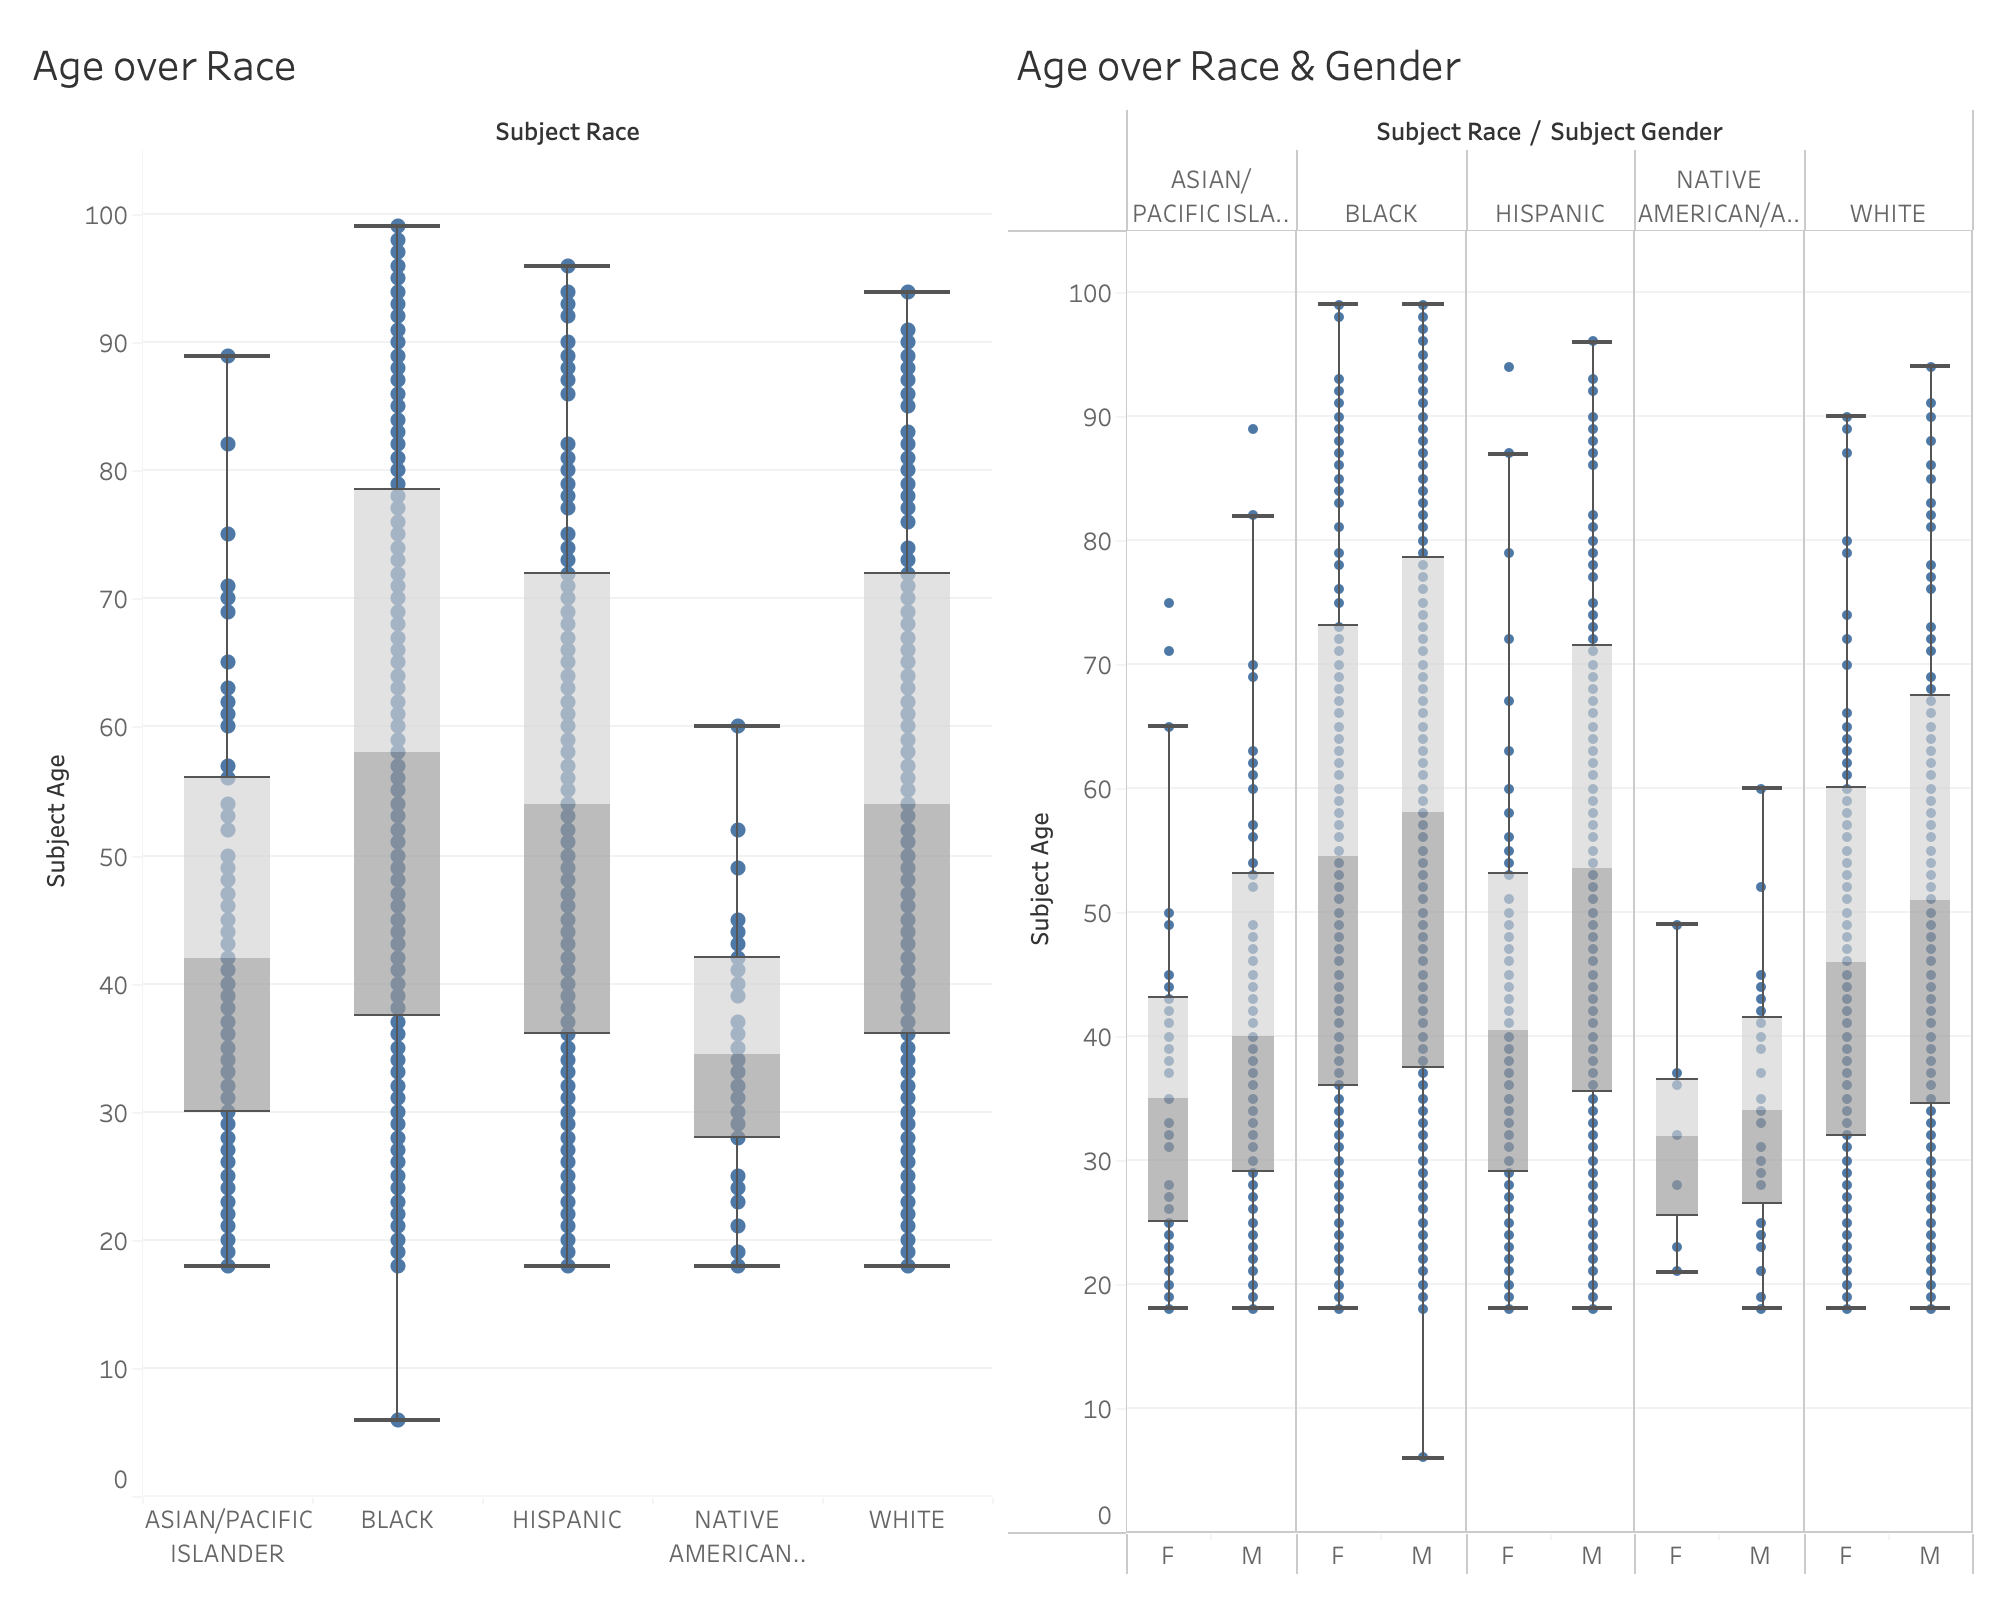
\includegraphics[scale=0.30]{image1.png}
\caption{Box and whisker plot of subject age over race and gender.}
\label{fig:subjage}
\end{figure}

From Figure \ref{fig:subjage}, we can see that among all the races, subjects of use of force cases that is Black, White, and Hispanic have higher age median than that of Asians and Native Americans. When we look into the gender, we can see that Hispanics have the largest difference between male and female. In the future, we can explore if the higher age median of race correlate with their larger proportion of population. Also for the Hispanic population, we would like to dig deeper to see if culture factor played a role.



\subsection{Influence of Different Environmental Conditions on Use of Force Cases for each Subject Race}

In this section, we plot a horizontal barchart for each environmental condition. In each barchart, we plot the percentage of cases happening under different conditions for each race.

\begin{figure}[h]
\centering
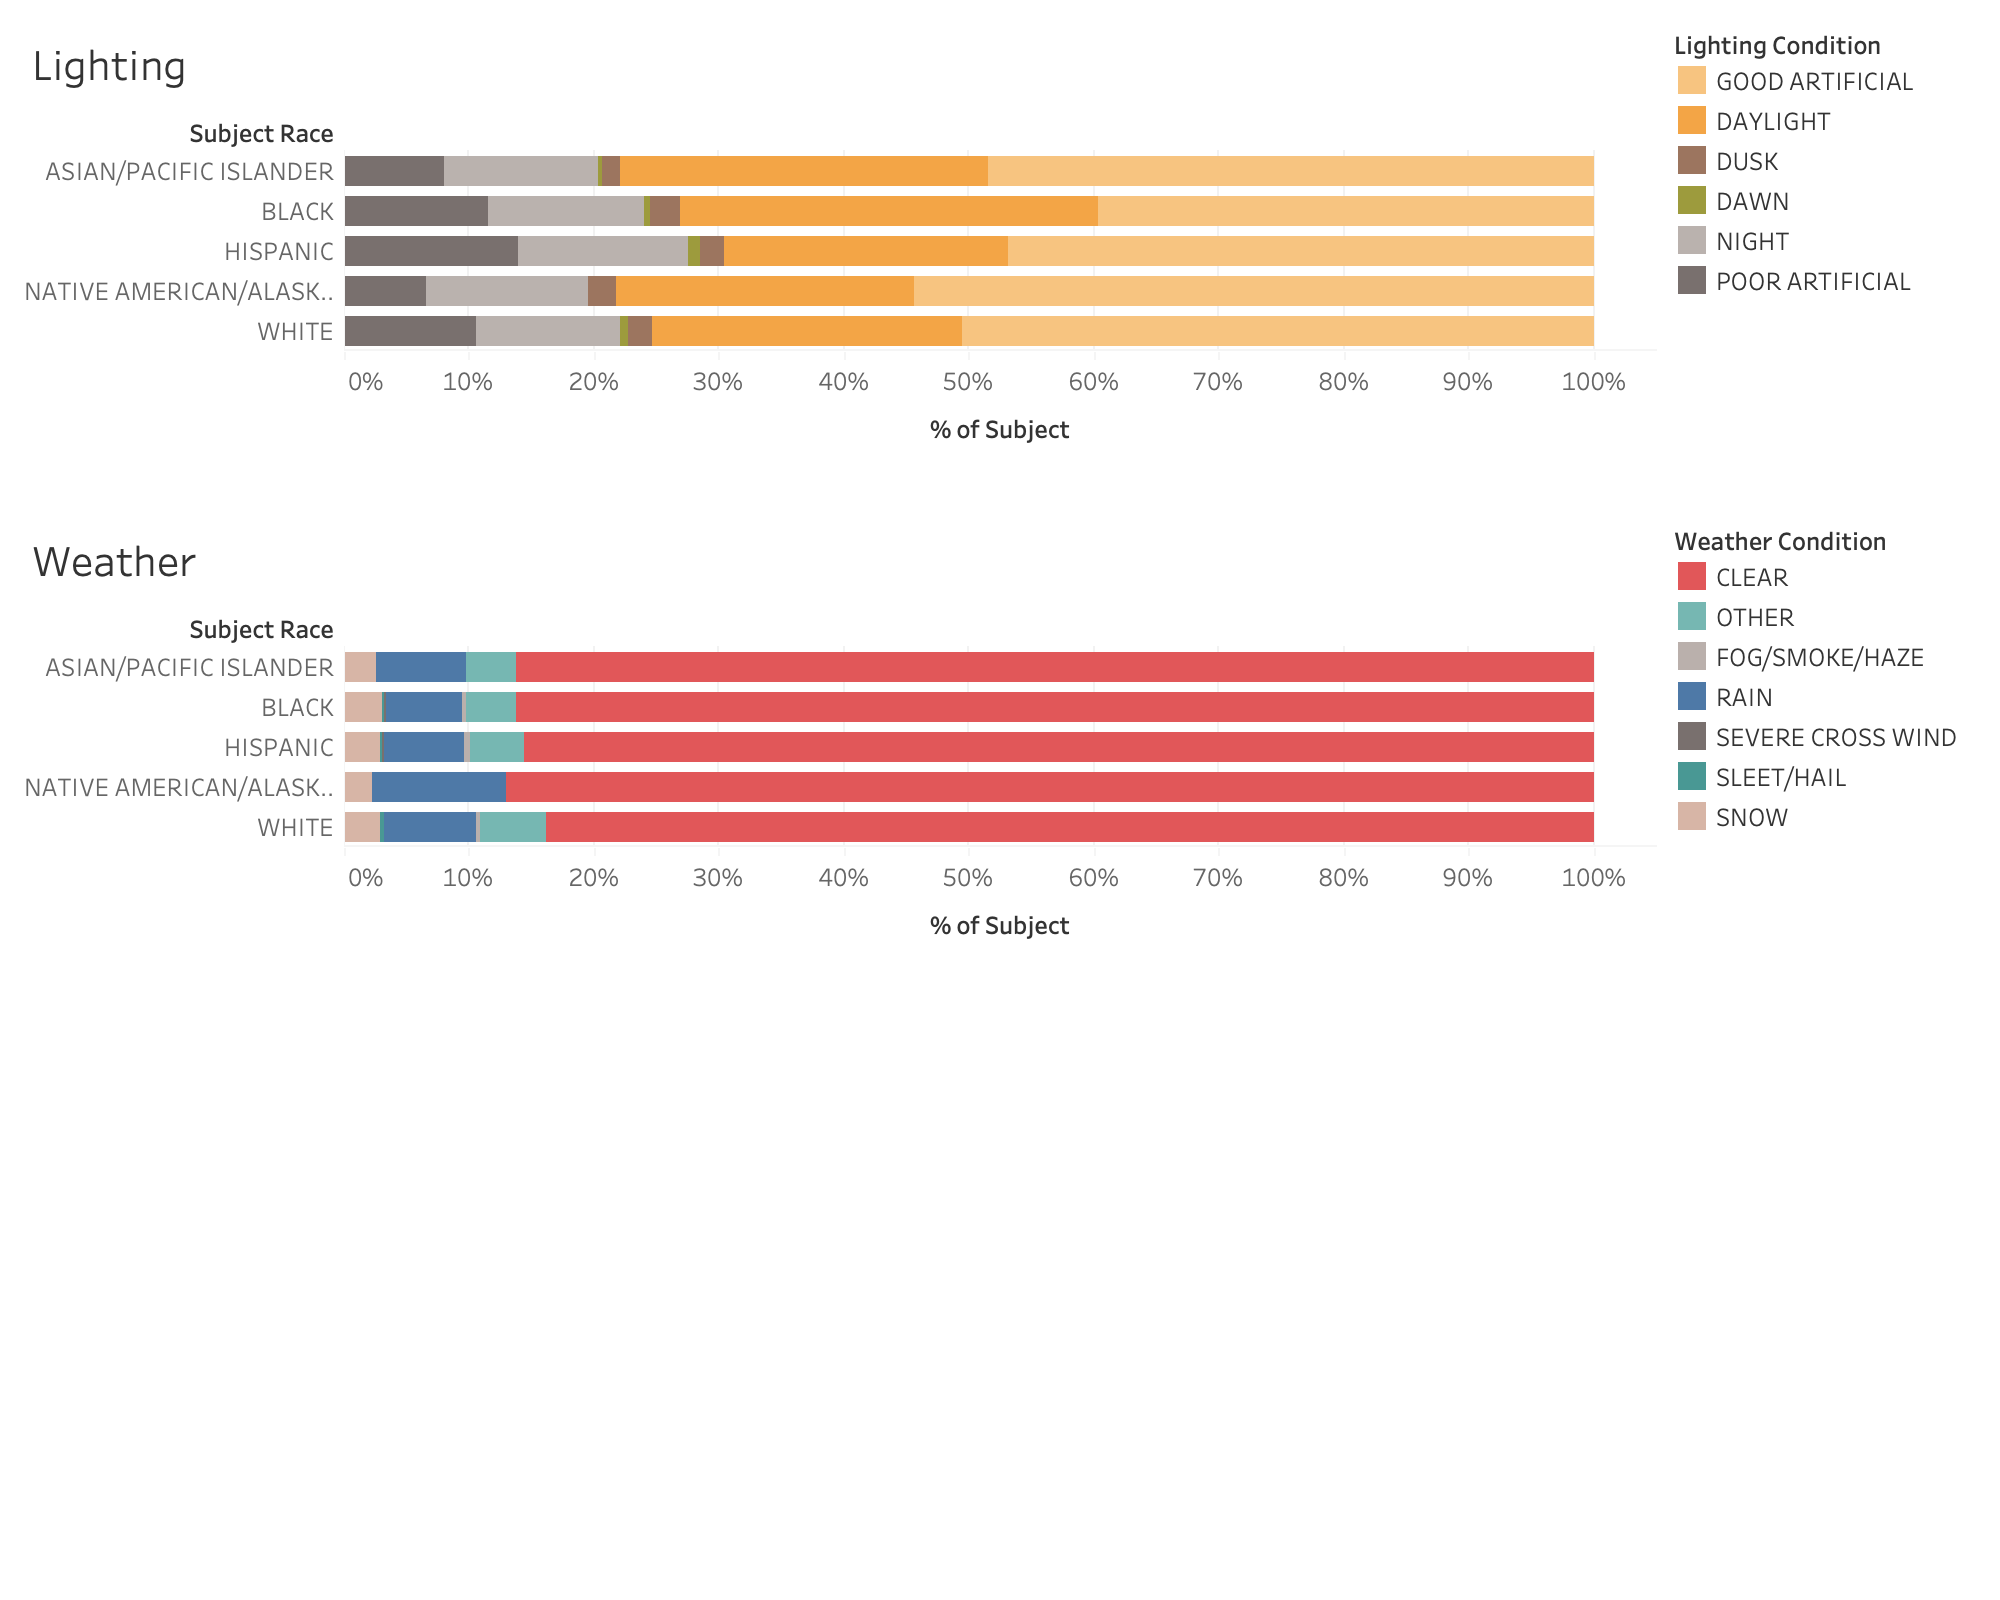
\includegraphics[scale=0.35]{image2.png}
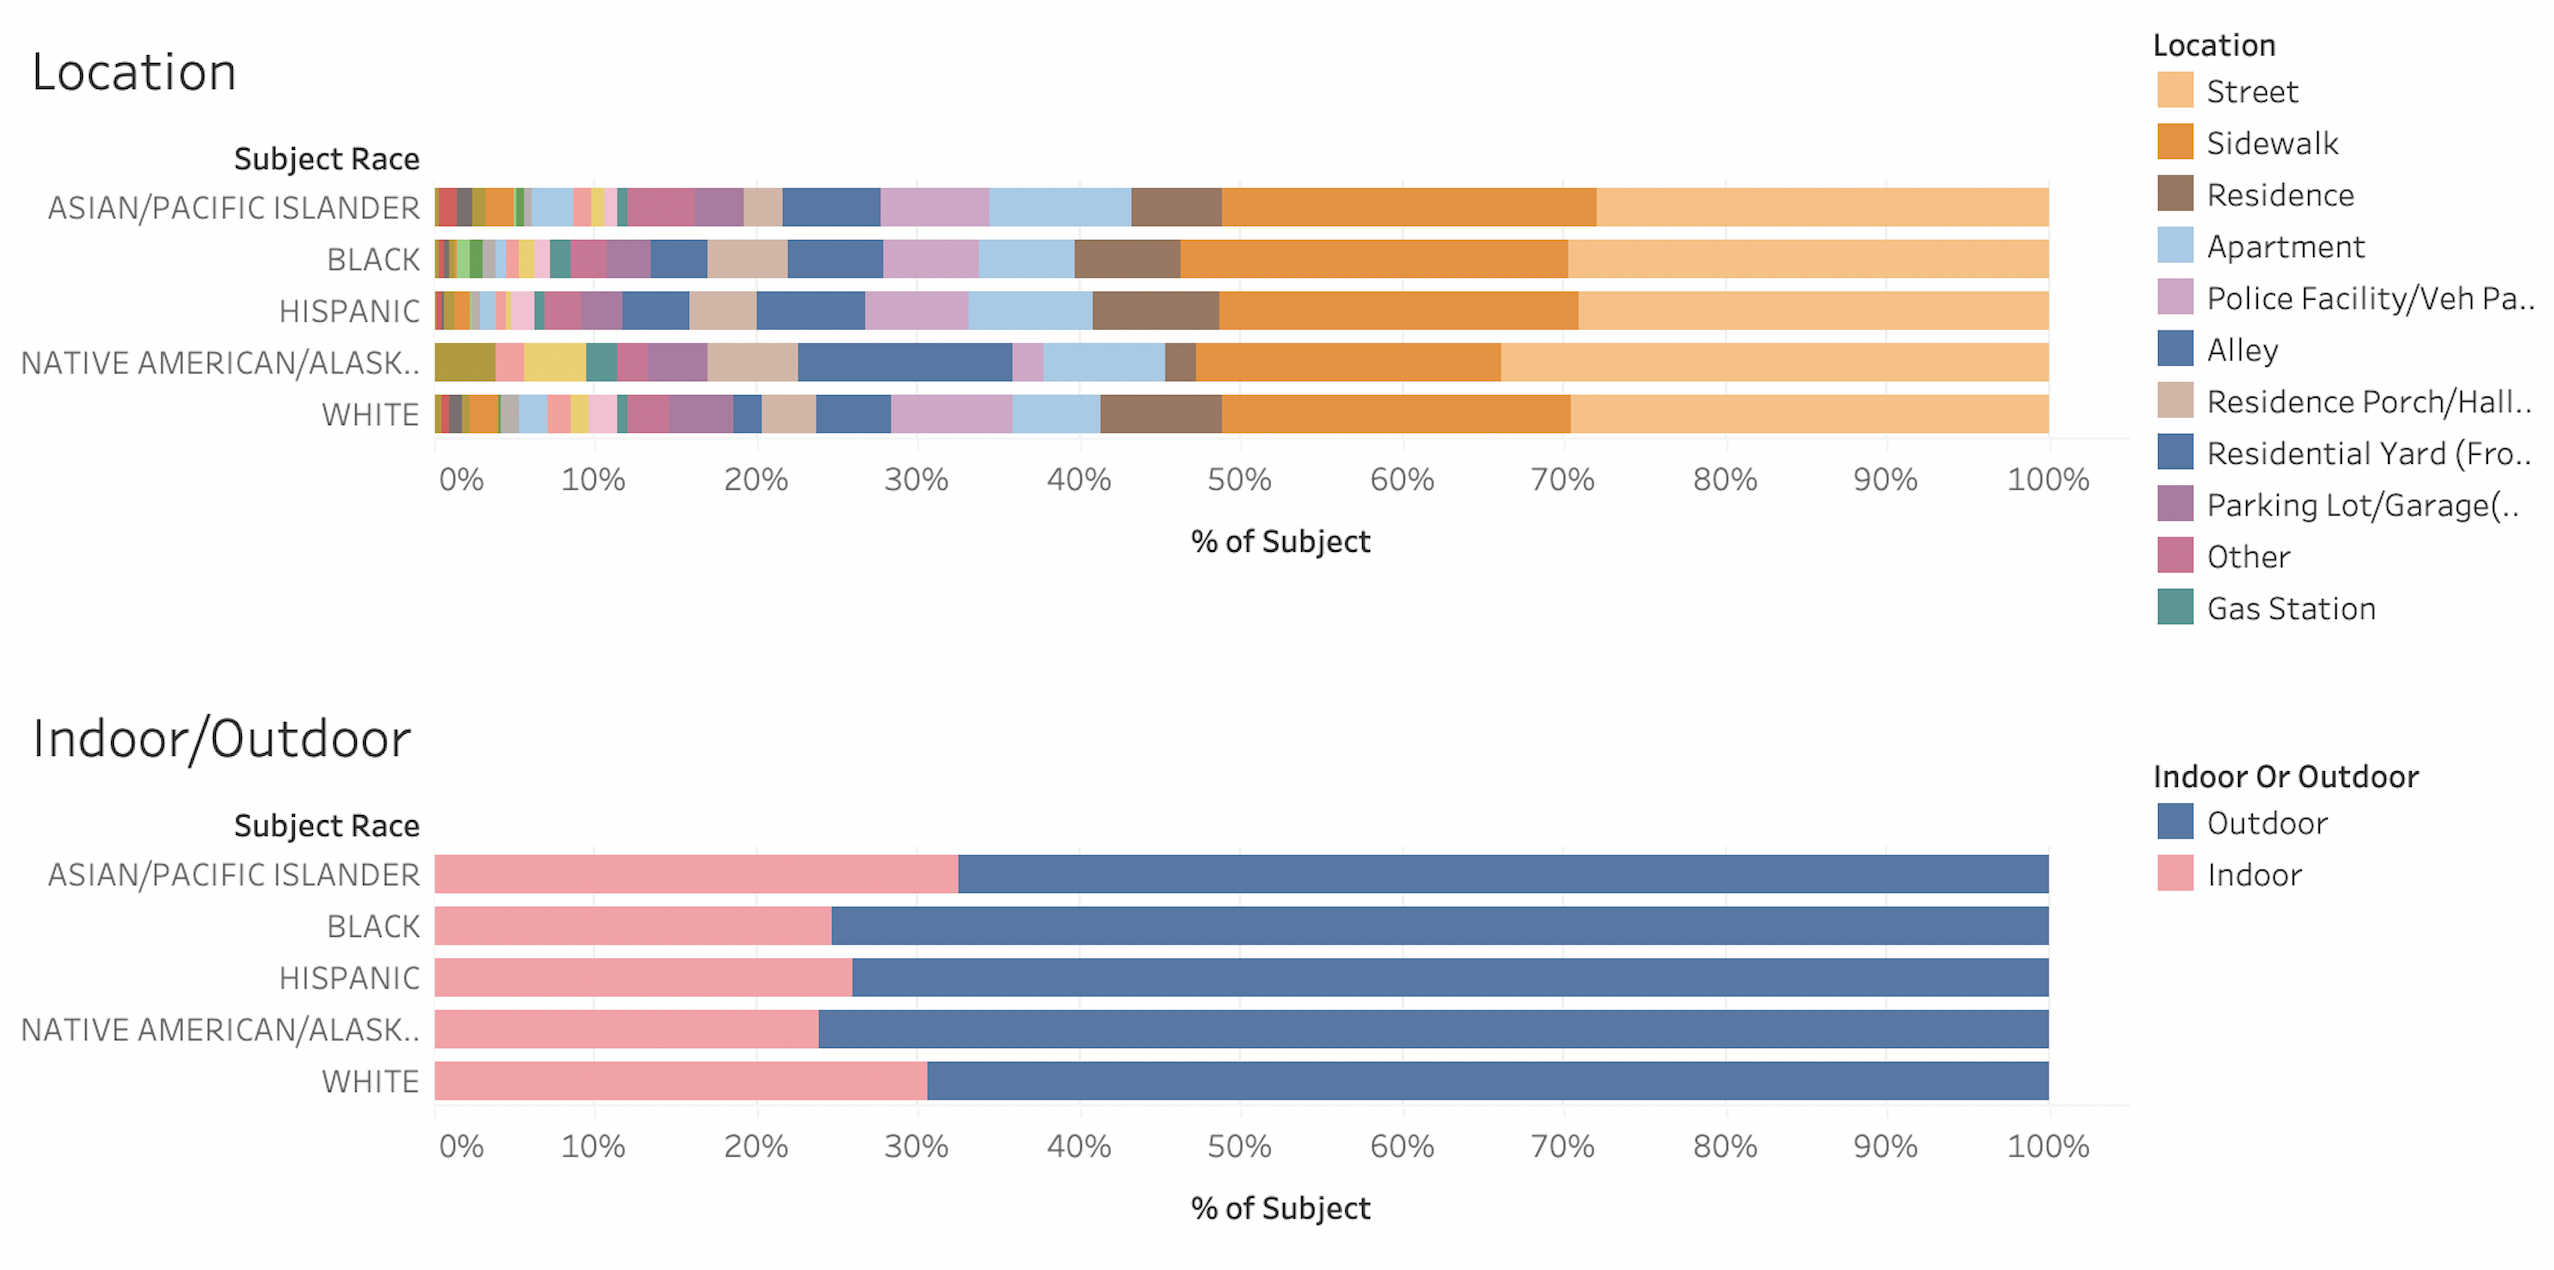
\includegraphics[scale=0.35]{image4.png}
\caption{Barchart of the frequency of police use of force cases in different environmental conditions (lighting, weather, location, indoors/outdoors) over each race}
\label{fig:conds}
\end{figure}


The four charts in Figure \ref{fig:conds} reflect the occurrence of use of force cases under different four conditions (Lighting, Indoor/Outdoor, Weather, Location). In terms of location. we can see that the majority of use of force cases happened in the street and on sidewalks. Most cases happen outdoors rather than indoors. Daylight and good artificial light, both of which can provide a better vision (brighter conditions) outrace the lighting conditions that provided worse vision. (darker conditions) The weather condition is almost dominated by clear weather. We don't know if these conditions are independent. Intuitively, clear weather and (daylight + good artificial) both imply better ability to see, while (sidewalk + street) and outdoor both imply a broader space. Further PCA (principal component analysis) might have us draw a better conclusion on this. What's more, race seems independent to the effect of these environmental factors.



\subsection{Cross Race Use of Force}

In this section, we created a bubble plot depicting the different combinations of officer race and subject race for police use of force cases.

\begin{figure}[h]
\centering
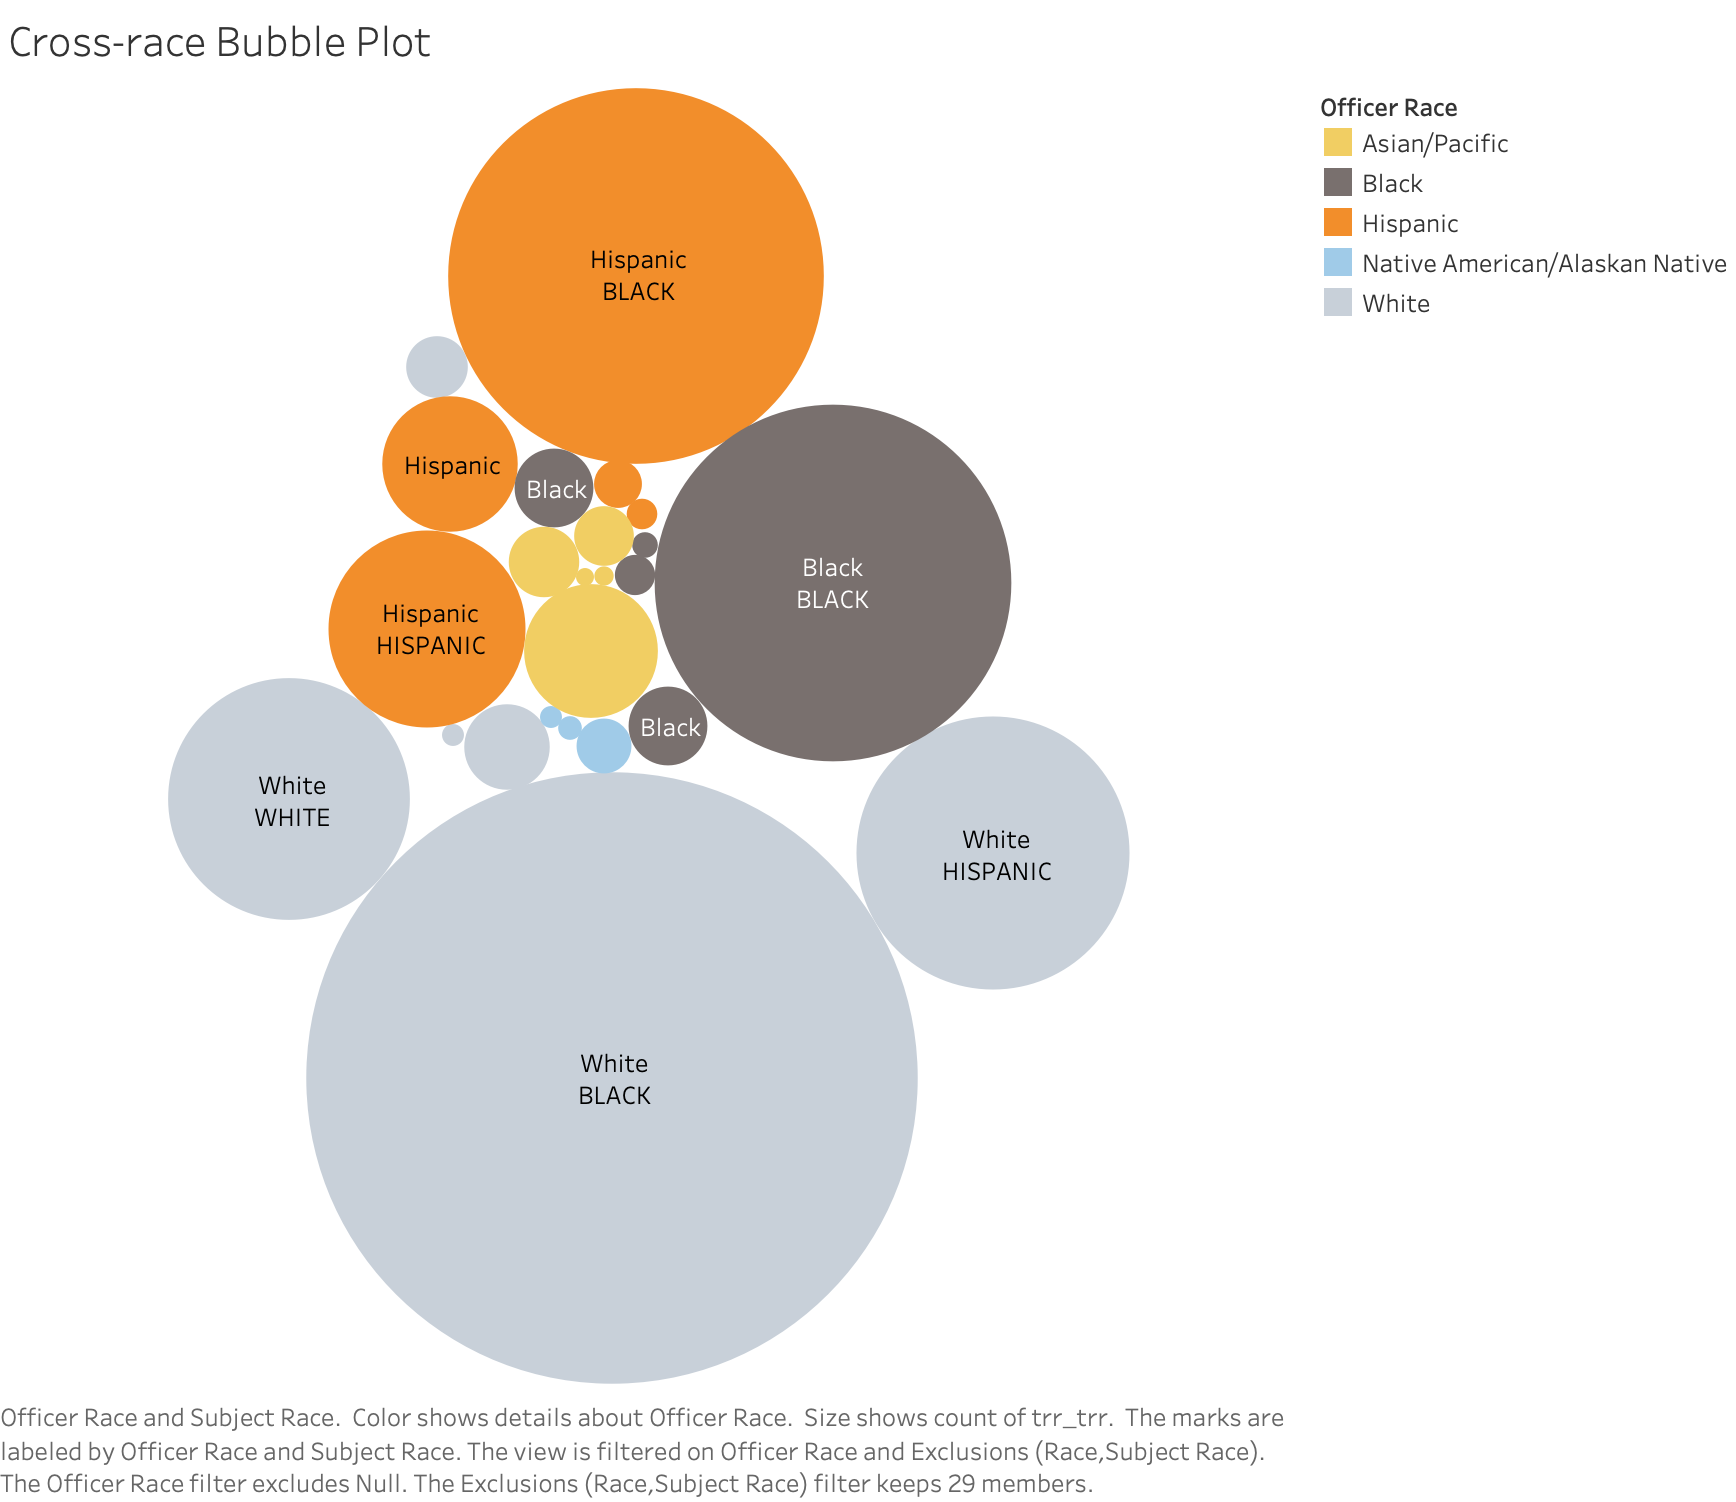
\includegraphics[scale=0.44]{image3.png}
\caption{Bubble plot depicting cross-race use of force cases. Each bubble contains the officer race (at the top) and the subject race (capitalized, at the bottom). The size of the bubble shows a visualization of count of use force cases. The plot filtered out cases where officer race is Null. Furthermore, the plot only kept the top 29 most common combinations.}
\label{fig:crossrace}
\end{figure}


By looking at Figure \ref{fig:crossrace}, we can see that top three cross race combinations are white officer to black subject, black officer to black subject, and hispanic officer to black subject. Surprisingly and unexpectedly, we found that black officer to black subject is one of the top three combinations. This leads us to consider the case of discrimination happening in the same race. Alternatively, this phenomenon may be explained by the fact that black subjects have the higher crime rates, so the occurrence of this situation is solely reflecting the portion of each race of officers in the population of officers.



\subsection{Barchart Comparing Use of Force Cases on each Race and Percentage of Population for each Race}

In this section, we plot a barchart of the percentage of the population of each race compared the total population. We also plot a barchart of the percentage of subjects of each race in police use of force cases compared to the total use of force subjects. We combined these two into a single barchart, making it easy to visualize the percentage comparisons.

\begin{figure}[h]
\centering
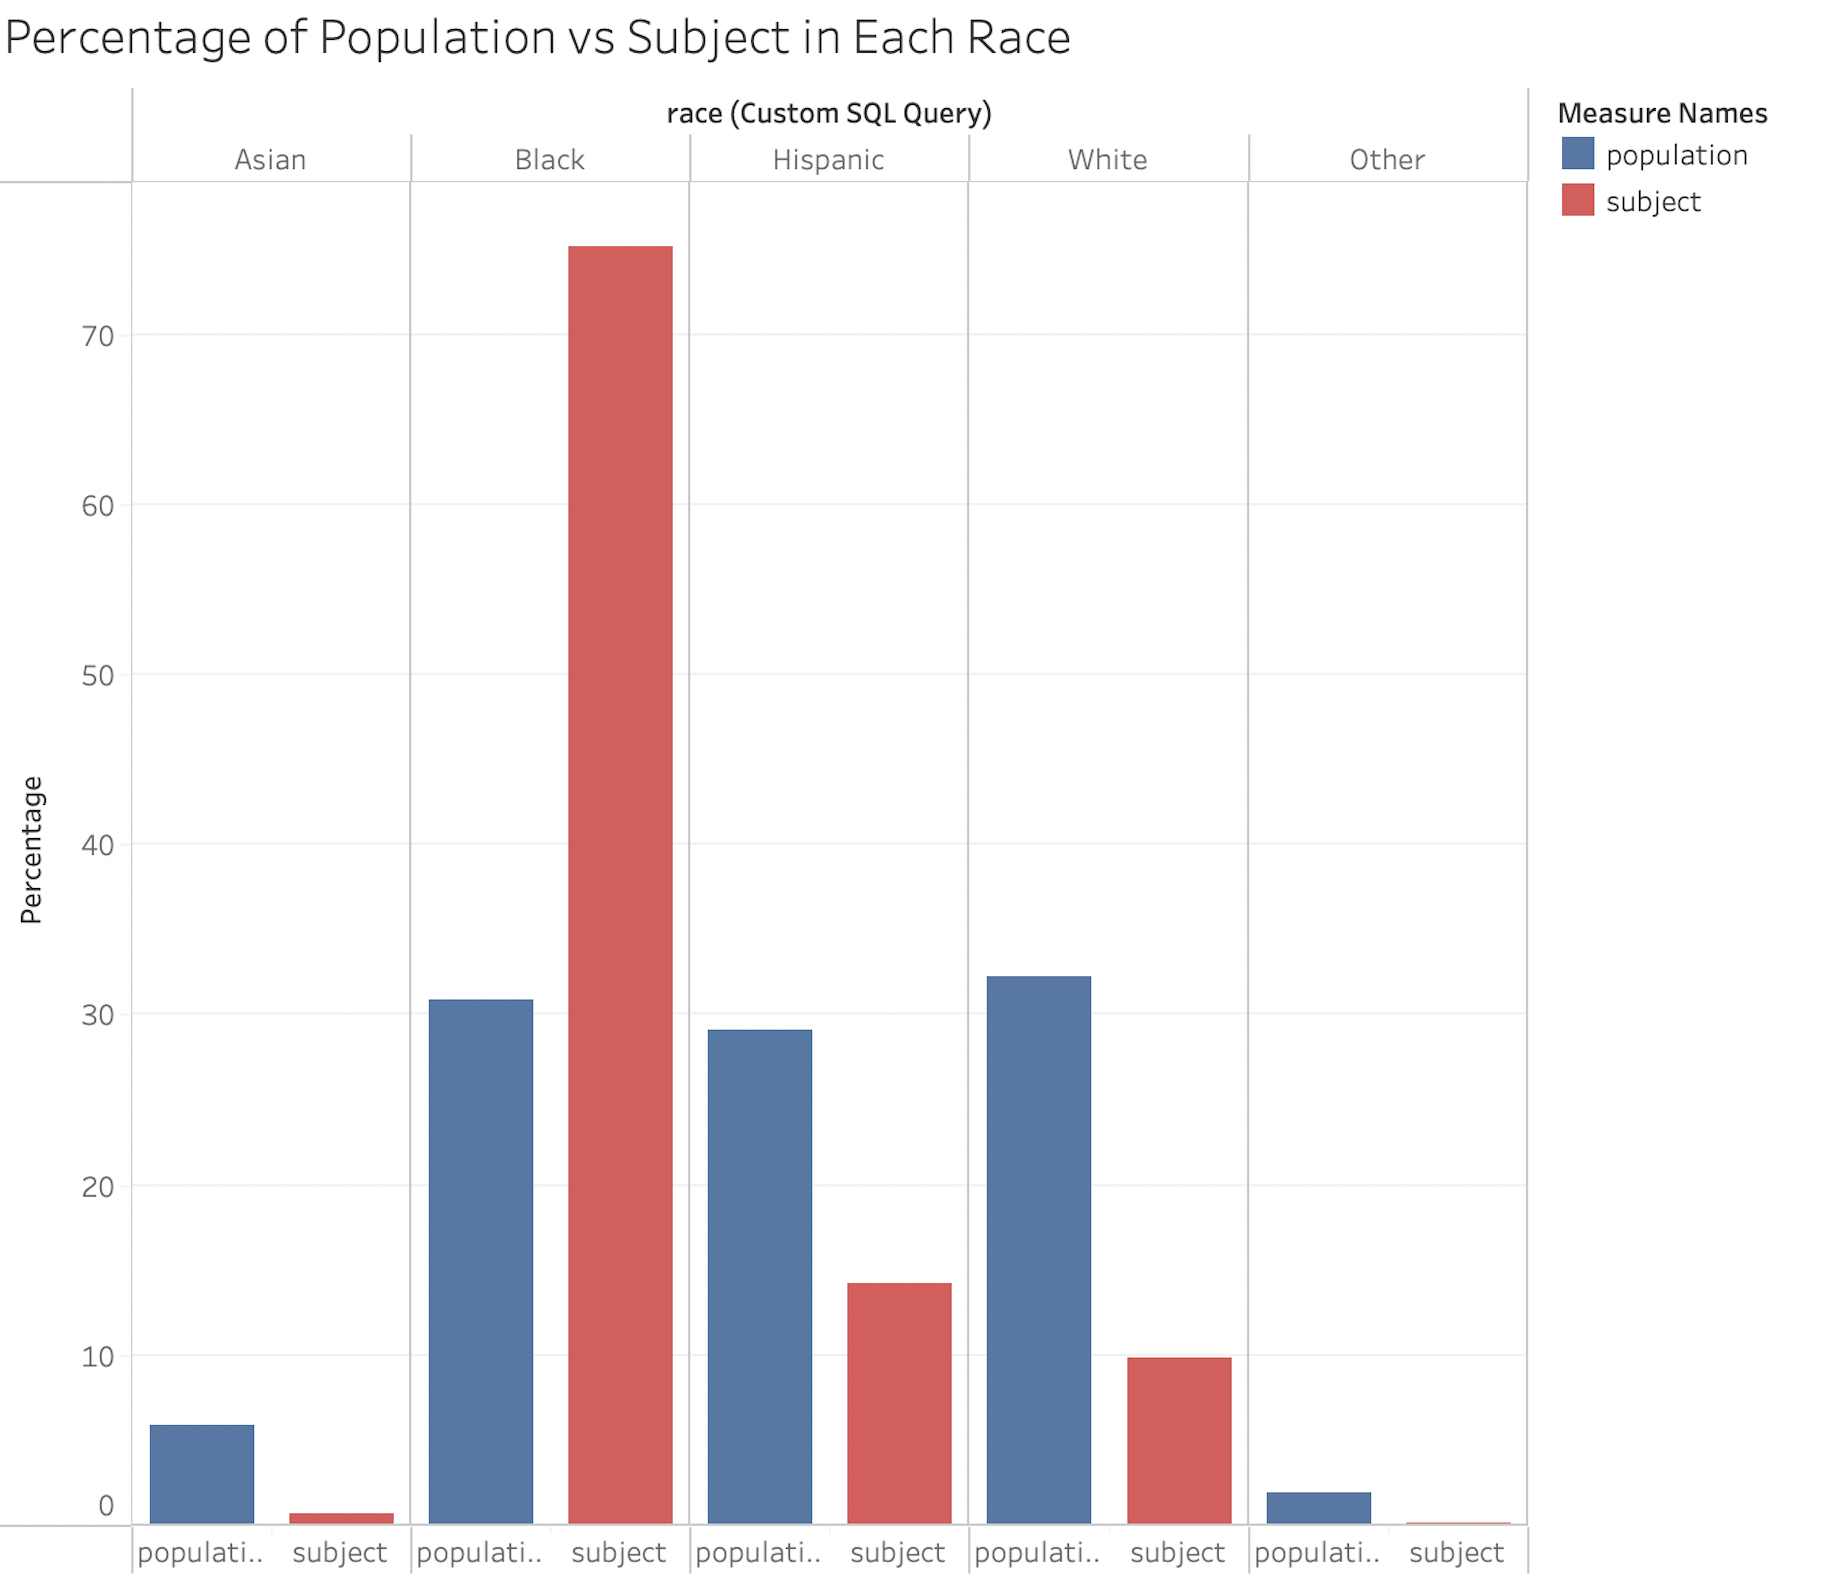
\includegraphics[scale=0.44]{image5.png}
\caption{Barcharts of (1) the percentage of the population of each race compared to the total population and (2) the percentage of use of force cases on subjects of each race compared to total use of force cases. The blue bar on the left represents the portion of race in the total population and the red bar on the right represents the portion of race in all subjects.}
\label{fig:population}
\end{figure}


From Figure \ref{fig:population}, we can observe that Black, Hispanic, and White make up the majority of the population, and they have almost the same portion in the population but at the same time, Black subjects account for more than 70 percentage of all subjects, while hispanic and white each accounts for only about 10-15 percentage of subjects. This result brings us to the existence of racial discrimination among police officers. We still need to do some investigation on the crime rate of each race in reality before we can make a solid conclusion on the existence of racial discrimination.




\section{Future Research Direction}





\section{Tableau Review}

In this section we will present an overview of the experience of our usage of Tableau, including what we believe to be advantages and disadvantages of the software.

\subsection{Advantages}

\begin{enumerate}

\item Tableau provides great visualiations and an intuitive user interface for handling these data tasks. The built-in graphs are easy to use and the software makes it easy to switch between different graphs. The software also makes sure that we are using the correct data values for different types of graphs.

\item Once connected, exploring and processing the data becomes an easy task. The software provides an overview of all the tables and the fields of each table. Table joining and field filtering is also straightforward.

\item Tableau makes it hard to make mistakes because it restricts the way we can visualize data. In other words, it won't allow us to use a certain type of graph unless our data satifies all constraints.

\item Tableau provides the capability to export workbooks. These workbooks are represented as structured XML data internally and this allows it to be checked into source control, making it easy to track version history.

\end{enumerate}

\subsection{Disadvantages}

\begin{enumerate}

\item Tableau's license is rather difficult to setup, even being a student. It requires us to upload our student IDs and wait for verfication. This process can fail unless the photo is taken clearly.

\item Connecting Tableau to a remote server is easy, but the connection relies heavily on the internet bandwidth. In most cases, the connection is not stable and the visualization tasks are extremely slow.

\item Connecting Tableau with local Postgres is hard. It requires us to download a specific driver to connect the software with the database and requires us to enter specific information for the connection. The error messages that are associated with the failures to connect are counter-intuitive and provide no information as to why the connection is failing, making it impossible to debug. We spent hours on the connection problems alone.

\end{enumerate}


\end{document}
